%%%%%%%%%%%%%%%%%%%%%%%%%%%%%%%%%%%%%%%%%%%%%%%%%%%%%%%%%%%%%%%%%%%%%%%%%%%%%%%%%%
\begin{frame}[fragile]\frametitle{}
\begin{center}
{\Large Introduction}
\end{center}
\end{frame}


%%%%%%%%%%%%%%%%%%%%%%%%%%%%%%%%%%%%%%%%%%%%%%%%%%%%%%%%%%%%%%%%%%%%%%%%%%%%%%%%%%
\begin{frame}[fragile]\frametitle{Why 'Go' after Reinforcement Learning?}

\begin{center}
\includegraphics[width=0.5\linewidth,keepaspectratio]{rl12}

\includegraphics[width=0.5\linewidth,keepaspectratio]{rl13}

Alpha Go (4) vs Lee Sedol (1)
\end{center}

\end{frame}

%%%%%%%%%%%%%%%%%%%%%%%%%%%%%%%%%%%%%%%%%%%%%%%%%%%%%%%%%%%%%%%%%%%%%%%%%%%%%%%%%%
\begin{frame}[fragile]\frametitle{Brief History}

\begin{center}
\includegraphics[width=\linewidth,keepaspectratio]{rl17}
\end{center}

{\tiny (Ref: But what is Reinforcement Learning? | Reinforcement Learning Part-1 - Rajtilak Pal (M. Tech in AI, IIT Ropar))}
\end{frame}

%%%%%%%%%%%%%%%%%%%%%%%%%%%%%%%%%%%%%%%%%%%%%%%%%%%%%%%%%%%%%%%%%%%%%%%%%%%%%%%%%%
\begin{frame}[fragile]\frametitle{Whats in RL?}

\begin{itemize}
\item   RL is not a new set of algorithms but a different way of structuring and solving problems. It is applicable only when such a structure is present.
\item   There are key entities in RL: Agent, Action, Environment, Reward, and States.
\end{itemize}

\begin{center}
\includegraphics[width=\linewidth,keepaspectratio]{rl1}
\end{center}

\end{frame}

%%%%%%%%%%%%%%%%%%%%%%%%%%%%%%%%%%%%%%%%%%%%%%%%%%%%%%%%%%%%%%%%%%%%%%%%%%%%%%%%%%
\begin{frame}[fragile]\frametitle{Whats in RL?}

\begin{itemize}
\item   The problem definition occurs within the environment. The environment consists of states, represented by variables. When an action is taken, the states change. A 'model' (if present) evaluates the favorability of the action and assigns a reward (positive or negative). After executing the action, the environment returns the new state variables and the corresponding reward.
\item   The Agent is the algorithm or strategy chosen to solve the problem. Various strategies can be applied to interpret the environment and maximize rewards. The agent selects actions it predicts will yield the highest reward. Initially, it takes random actions in a phase called Exploration. Once it learns which actions generally lead to favorable outcomes within the black-box environment, it transitions to Exploitation, where it prioritizes those actions for maximum rewards. These strategies, when implemented in code, are called Policies.
\end{itemize}



\end{frame}


%%%%%%%%%%%%%%%%%%%%%%%%%%%%%%%%%%%%%%%%%%%%%%%%%%%%%%%%%%%%%%%%%%%%%%%%%%%%%%%%%%
\begin{frame}[fragile]\frametitle{What is Reinforcement Learning?}
Reinforcement Learning(RL) is a type of machine learning technique that enables an agent to learn in an interactive environment by trial and error using feedback from its own actions and experiences, to maximize cumulative rewards.

\begin{center}
\includegraphics[width=0.6\linewidth,keepaspectratio]{rl9}
\end{center}


\end{frame}

%%%%%%%%%%%%%%%%%%%%%%%%%%%%%%%%%%%%%%%%%%%%%%%%%%%%%%%%%%%%%%%%%%%%%%%%%%%%%%%%%%
\begin{frame}[fragile]\frametitle{The Reinforcement Learning Problem}

\begin{columns}
    \begin{column}[T]{0.5\linewidth}
		The objective of supervised learning is to be able to generalize or extrapolate in situations not present in the training dataset.

		\begin{center}
		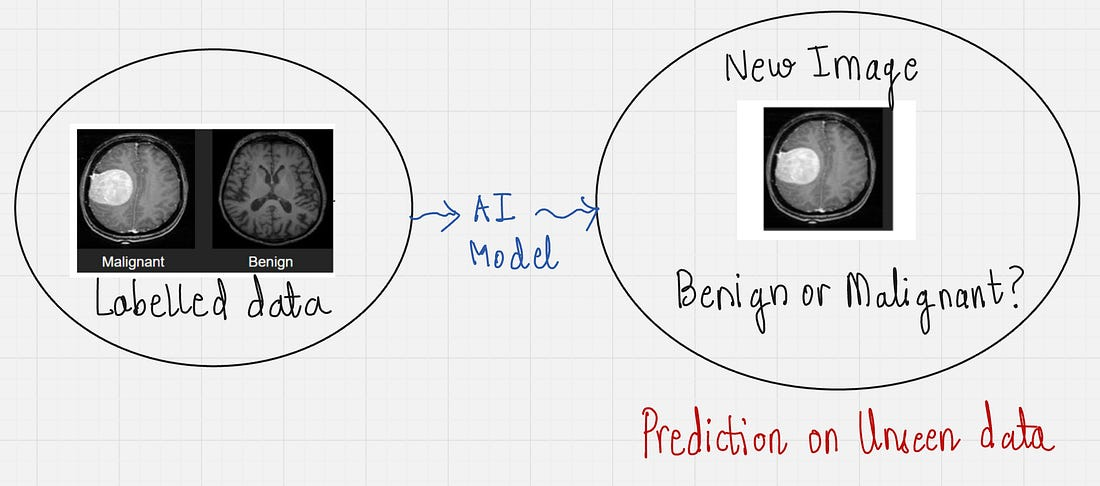
\includegraphics[width=\linewidth,keepaspectratio]{rl159}

		\end{center}

    \end{column}
    \begin{column}[T]{0.5\linewidth}
		Unsupervised learning finds structures that are hidden in collections of unlabeled data.

		\begin{center}
		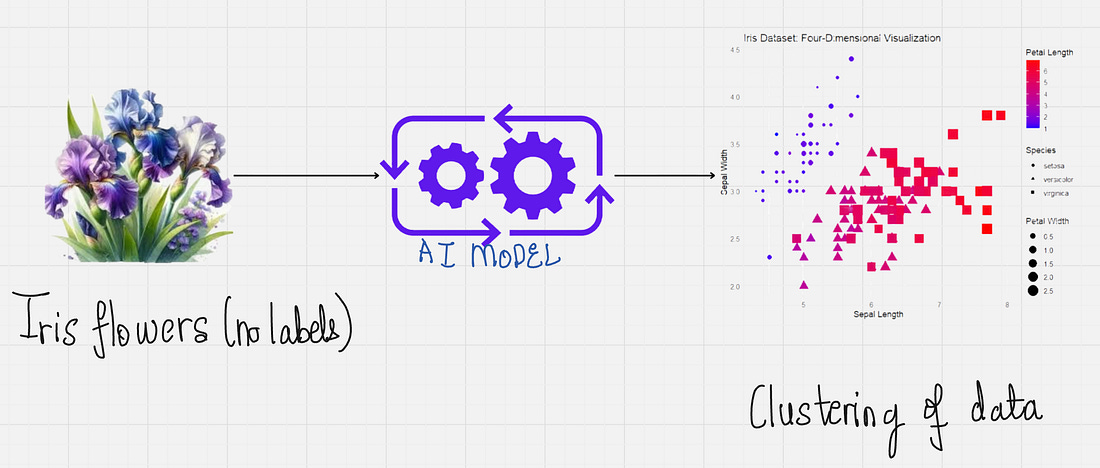
\includegraphics[width=\linewidth,keepaspectratio]{rl160}

		\end{center}
    \end{column}
  \end{columns}

{\tiny (Ref: Hands-on RL - Vizuara)}

\end{frame}

%%%%%%%%%%%%%%%%%%%%%%%%%%%%%%%%%%%%%%%%%%%%%%%%%%%%%%%%%%%%%%%%%%%%%%%%%%%%%%%%%%
\begin{frame}[fragile]\frametitle{The Reinforcement Learning Problem}

\begin{columns}
    \begin{column}[T]{0.5\linewidth}
		RL learns from interactions with the environment. Since there is no labeled data provided, it cannot converge to anything 'correct'.

		\begin{center}
		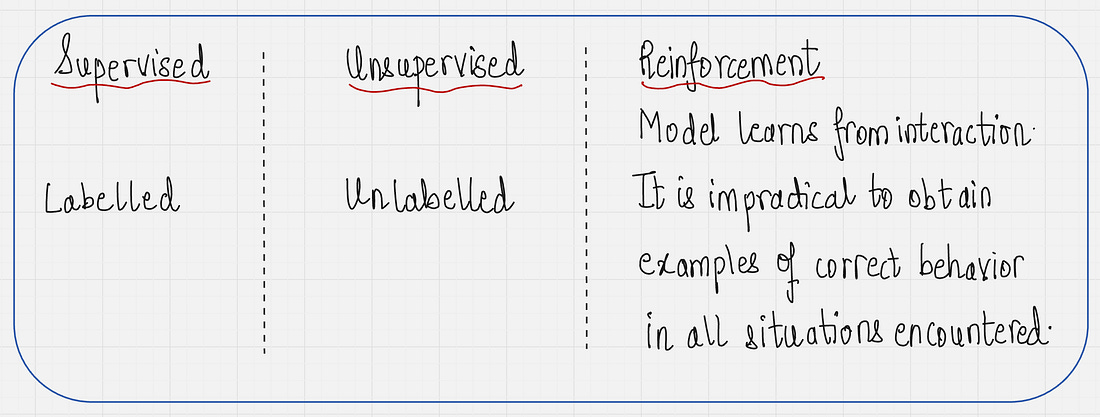
\includegraphics[width=\linewidth,keepaspectratio]{rl161}

		\end{center}

    \end{column}
    \begin{column}[T]{0.5\linewidth}
		In RL, the goal is to maximize a reward signal. 

		\begin{center}
		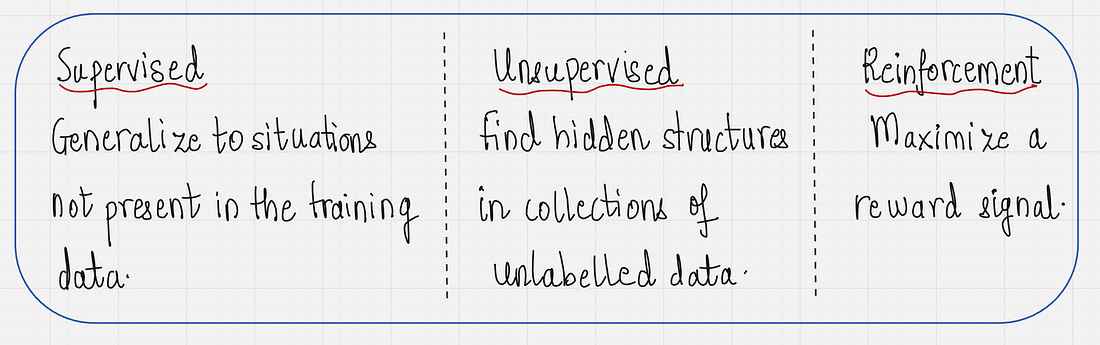
\includegraphics[width=\linewidth,keepaspectratio]{rl162}

		\end{center}
    \end{column}
  \end{columns}

{\tiny (Ref: Hands-on RL - Vizuara)}

\end{frame}

%%%%%%%%%%%%%%%%%%%%%%%%%%%%%%%%%%%%%%%%%%%%%%%%%%%%%%%%%%%%%%%%%%%%%%%%%%%%%%%%%%
\begin{frame}[fragile]\frametitle{What is Reinforcement Learning?}

\begin{center}
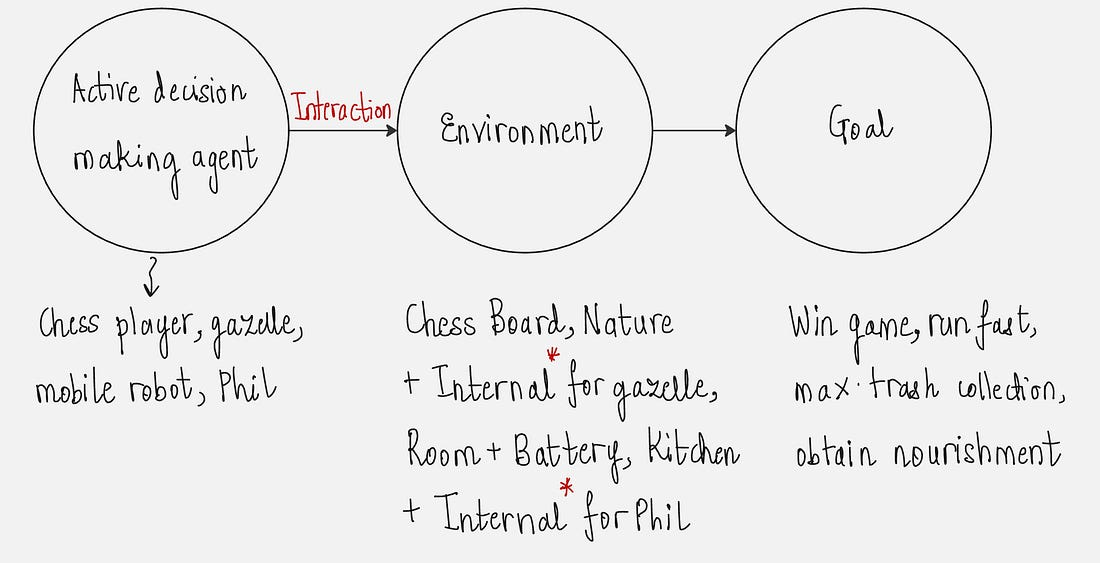
\includegraphics[width=\linewidth,keepaspectratio]{rl163}

{\tiny (Ref: Hands-on RL - Vizuara)}

\end{center}


\end{frame}

%%%%%%%%%%%%%%%%%%%%%%%%%%%%%%%%%%%%%%%%%%%%%%%%%%%%%%%%%%%%%%%%%%%%%%%%%%%%%%%%%%
\begin{frame}[fragile]\frametitle{The big picture}
\begin{itemize}
\item An agent (an AI) will learn from the environment by interacting with it (through trial and error) and receiving rewards (negative or positive) as feedback for performing actions.
\item Learning from interaction with the environment comes from our natural experiences.
\item Like, without any supervision, the child will get better and better at playing the game.
\end{itemize}

{\tiny (Ref: Chapter 1 of the Deep Reinforcement Learning Class with Hugging Face)}


\end{frame}

%%%%%%%%%%%%%%%%%%%%%%%%%%%%%%%%%%%%%%%%%%%%%%%%%%%%%%%%%%%%%%%%%%%%%%%%%%%%%%%%%
\begin{frame}[fragile]\frametitle{Elements of Reinforcement Learning}

Reinforcement Learning (RL) hinges on four key concepts that shape how agents learn to make decisions.

\begin{itemize}
\item Policy: Think of this as the agent�s instinct. It defines how the agent acts in any given situation�a direct mapping from states to actions.
\item Reward Signal: The heartbeat of RL. This is the immediate feedback�positive or negative�that tells the agent what�s desirable. Want to avoid pain or seek pleasure? That�s reward at play.
\item Value Function: Not everything is about the now. The value function helps the agent look ahead�estimating the total future reward it can expect from a state. Imagine a cricketer who underperforms early on but holds promise for future games�the short-term reward is low, but the long-term value is high.
\item Model of the Environment: Want to predict what happens next? That�s where a model comes in. It mimics how the environment behaves and can be used for planning (model-based) or skipped entirely (model-free).
\end{itemize}

{\tiny (Ref: Hands-on RL - Vizuara)}

\end{frame}

%%%%%%%%%%%%%%%%%%%%%%%%%%%%%%%%%%%%%%%%%%%%%%%%%%%%%%%%%%%%%%%%%%%%%%%%%%%%%%%%%
\begin{frame}[fragile]\frametitle{Game Example: Tic-Tac-Toe}

The goal? Design a player that not only competes, but learns to exploit weaknesses in its opponent�s strategy and maximize its own chances of winning.

Let�s break down the core building blocks behind this intelligent gameplay:

\begin{itemize}
\item State: Every possible layout of X�s and O�s on the 3x3 grid is a state. The board is the world our agent sees.
\item Policy: This is the agent�s game plan, a rulebook that says, �Given this board, play here.� It maps every state to the best possible move.
\item Value Function: Not all board positions are created equal. The value function assigns each state a number, an evolving estimate of how likely it is to win from that point. Think of it as the player�s intuition about how good a position really is.
\end{itemize}


\end{frame}



%%%%%%%%%%%%%%%%%%%%%%%%%%%%%%%%%%%%%%%%%%%%%%%%%%%%%%%%%%%%%%%%%%%%%%%%%%%%%%%%%
\begin{frame}[fragile]\frametitle{Game Example: Tic-Tac-Toe}

\begin{center}
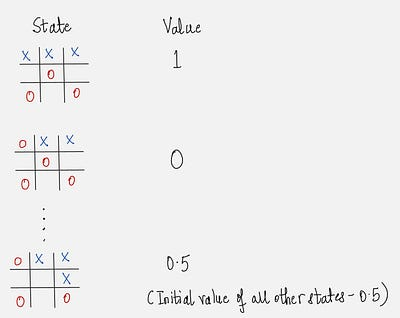
\includegraphics[width=0.8\linewidth,keepaspectratio]{rl164}

{\tiny (Ref: Hands-on RL - Vizuara)}

\end{center}

\end{frame}


%%%%%%%%%%%%%%%%%%%%%%%%%%%%%%%%%%%%%%%%%%%%%%%%%%%%%%%%%%%%%%%%%%%%%%%%%%%%%%%%%
\begin{frame}[fragile]\frametitle{Game Example: Tic-Tac-Toe}

\begin{itemize}
\item The value corresponding to the states will change as our agent plays the game more number of times.
\item Now, let us see how we modify the value function estimates as we play the game more number of times so that they reflect the true probabilities.
\item Let us say we are playing �X� and we are in the state given below:
\end{itemize}

\begin{center}
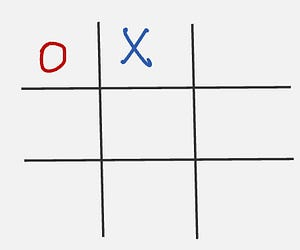
\includegraphics[width=0.5\linewidth,keepaspectratio]{rl165}

{\tiny (Ref: Hands-on RL - Vizuara)}

\end{center}

\end{frame}

%%%%%%%%%%%%%%%%%%%%%%%%%%%%%%%%%%%%%%%%%%%%%%%%%%%%%%%%%%%%%%%%%%%%%%%%%%%%%%%%%
\begin{frame}[fragile]\frametitle{Game Example: Tic-Tac-Toe}

\begin{itemize}
\item Now to play our next move, we look at all possible next states and select the one with the highest probability.
\item All the possible next states are given below:
\end{itemize}

\begin{center}
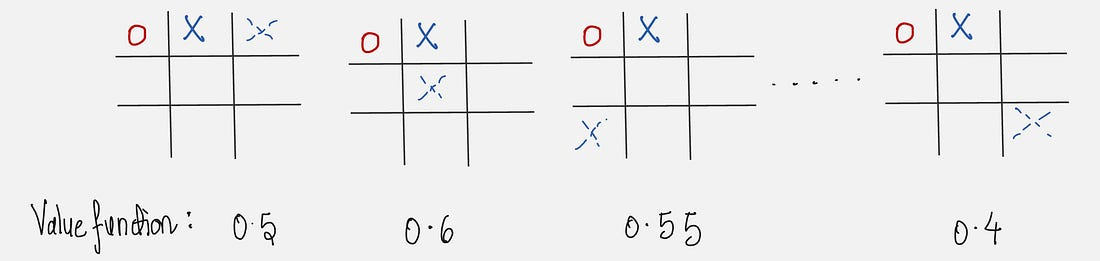
\includegraphics[width=0.8\linewidth,keepaspectratio]{rl166}

{\tiny (Ref: Hands-on RL - Vizuara)}

\end{center}


\begin{itemize}
\item We select the move which has a value function of 0.6. This is called exploitation, selecting the state with the greatest value.
\item But sometimes we select randomly from the available states so that we can experience states that you otherwise might not see.
\item For example, we can select the state with a value function of 0.4. This is called as exploration.
\end{itemize}
\end{frame}

%%%%%%%%%%%%%%%%%%%%%%%%%%%%%%%%%%%%%%%%%%%%%%%%%%%%%%%%%%%
\begin{frame}[fragile]\frametitle{Game Example: Tic-Tac-Toe}
\begin{columns}
    \begin{column}[T]{0.5\linewidth}
      \begin{itemize}
		\item While we are playing, we change the value of the states we find ourselves in. 
		\item We make them more accurate estimates of the probability of winning.
		\item After each greedy move (exploitation), the current value of the earlier state is adjusted to be closer to the value of the latter state. 
		\item This is done by moving the earlier state value a fraction of a way towards the latter state. This is called backing up.
	  \end{itemize}

    \end{column}
    \begin{column}[T]{0.5\linewidth}
		\begin{center}
		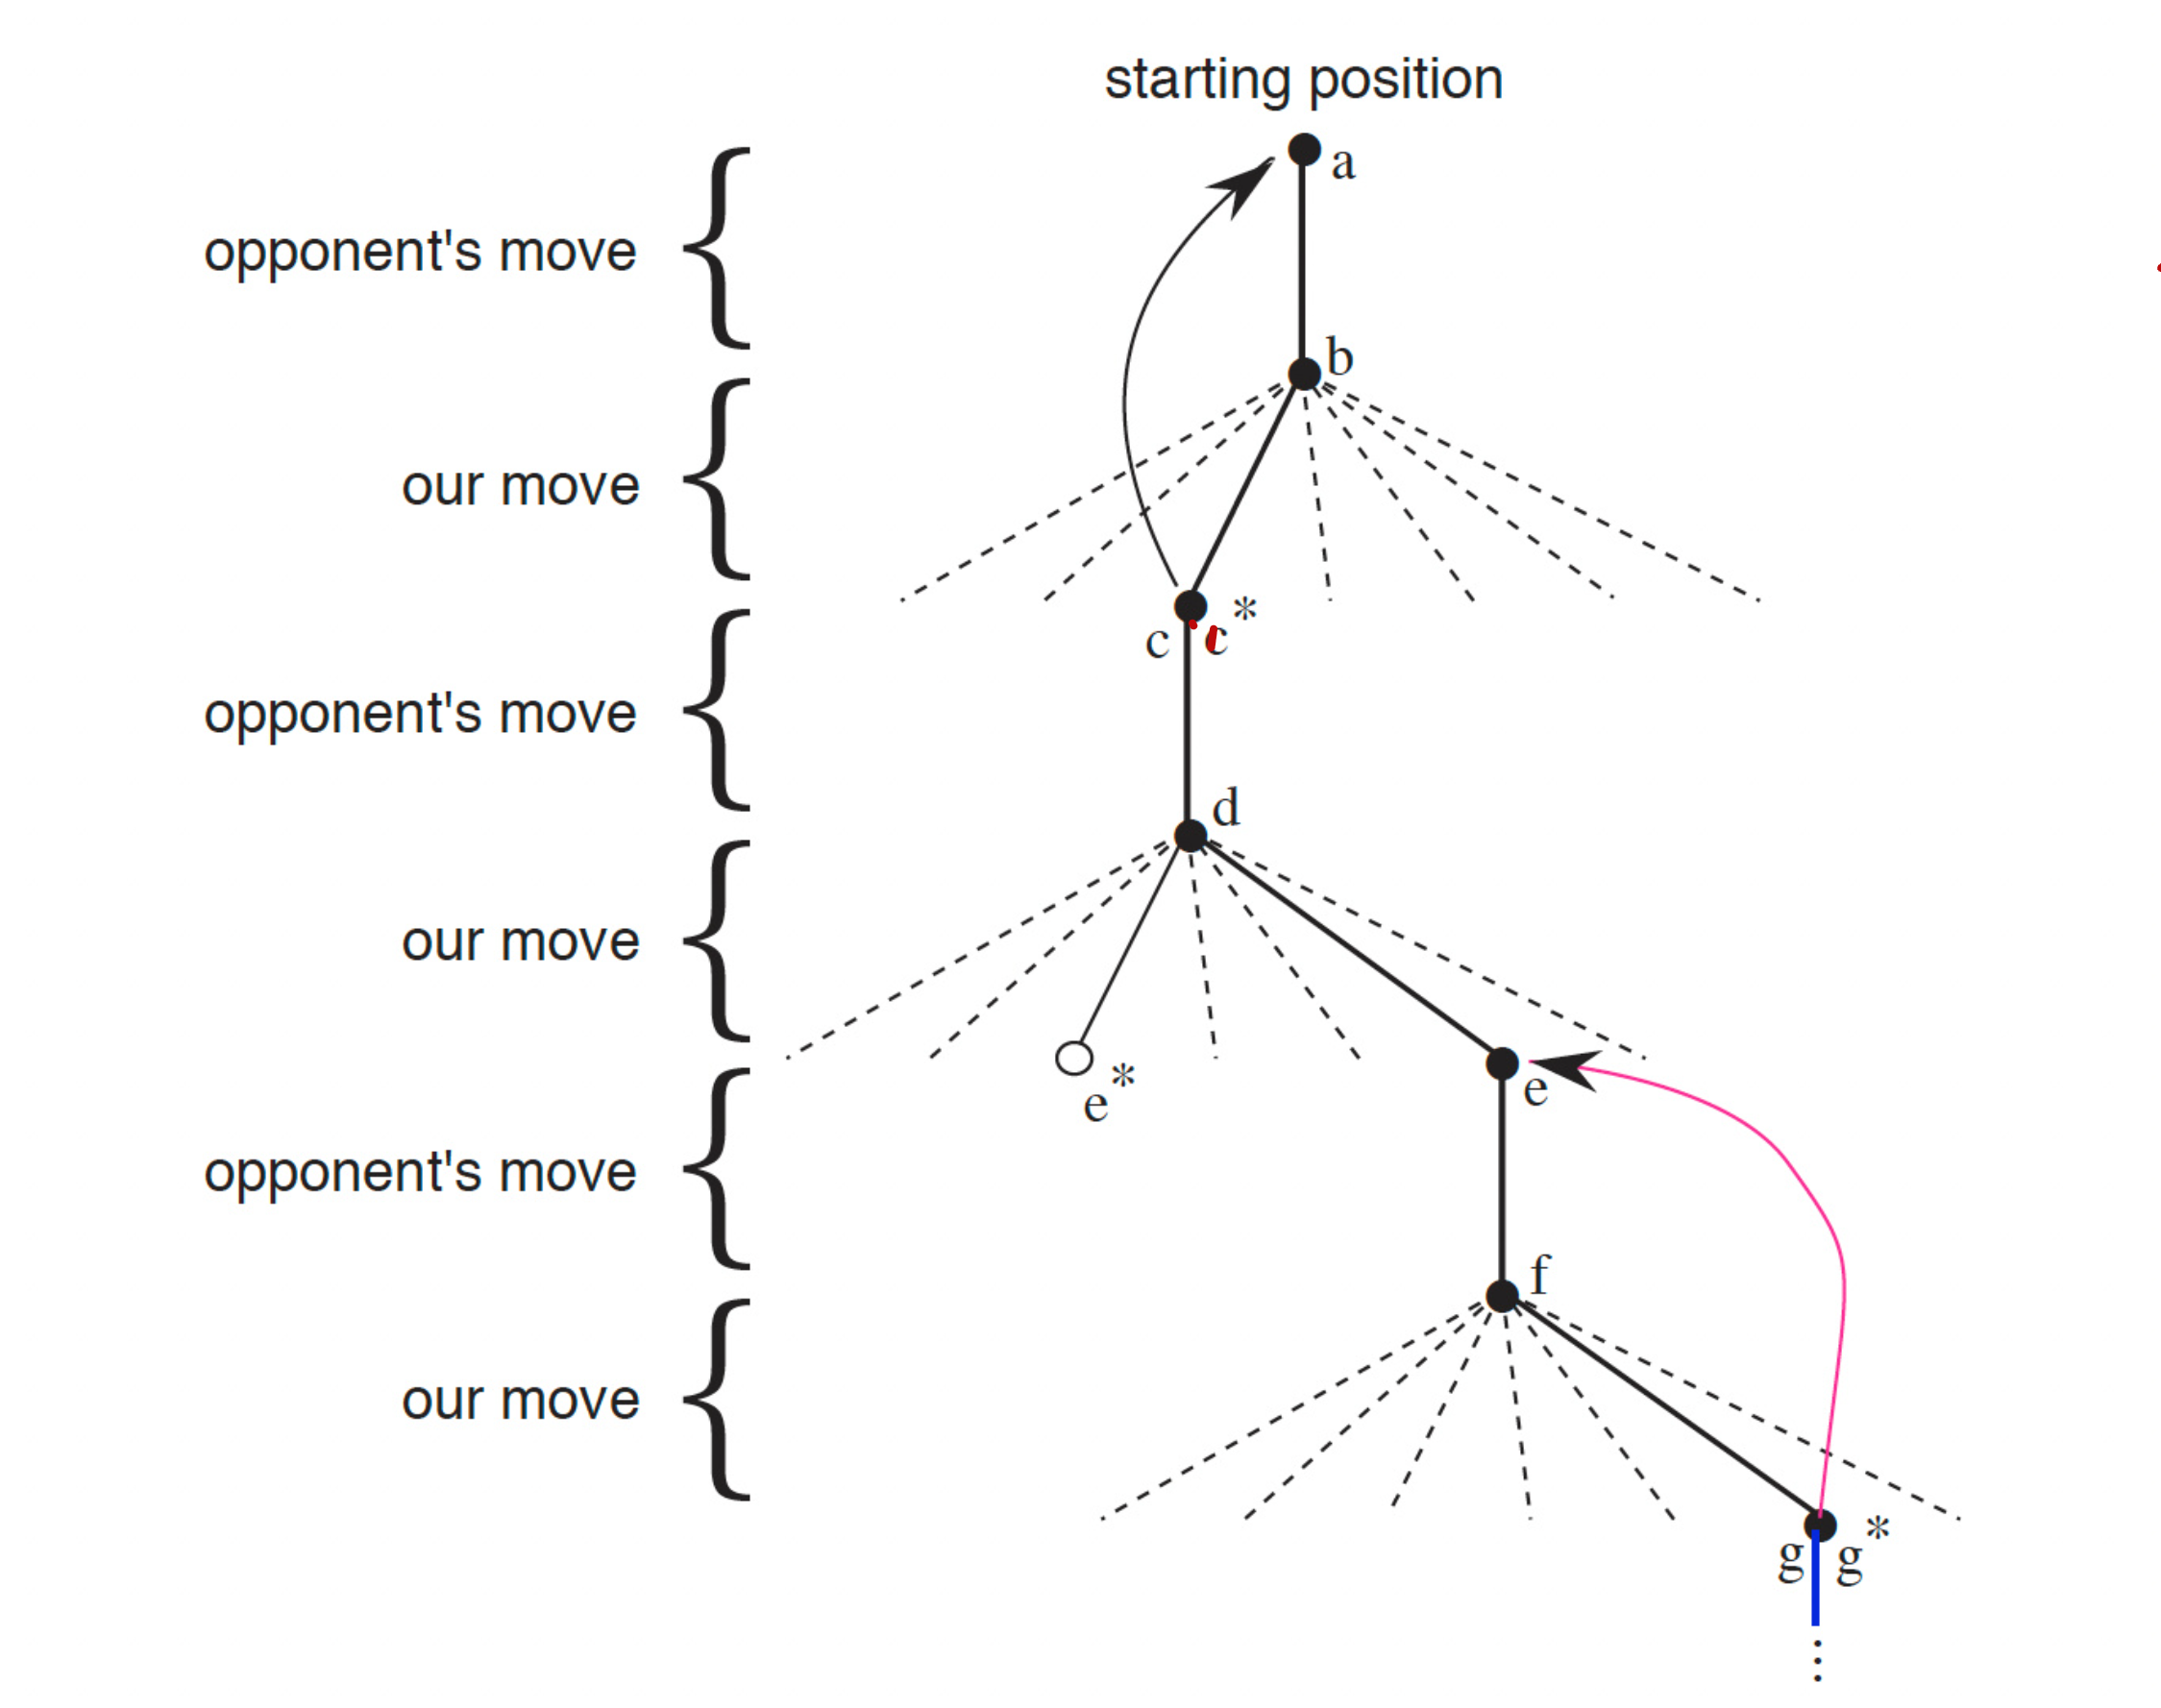
\includegraphics[width=0.8\linewidth,keepaspectratio]{rl167}

		{\tiny (Ref: Hands-on RL - Vizuara)}

		\end{center}
    \end{column}
  \end{columns}
\end{frame}

%%%%%%%%%%%%%%%%%%%%%%%%%%%%%%%%%%%%%%%%%%%%%%%%%%%%%%%%%%%%%%%%%%%%%%%%%%%%%%%%%
\begin{frame}[fragile]\frametitle{Game Example: Tic-Tac-Toe}
What did we learn from this example?

\begin{itemize}
\item In reinforcement learning, the learning happens by interacting with the environment/the opponent player.
\item There is a clear goal and correct behavior includes planning, especially delayed effects of one's choices.
\item This was an example of model-free reinforcement learning; we did not use any model of the opponent.
\end{itemize}

\end{frame}

%%%%%%%%%%%%%%%%%%%%%%%%%%%%%%%%%%%%%%%%%%%%%%%%%%%%%%%%%%%%%%%%%%%%%%%%%%%%%%%%%%
\begin{frame}[fragile]\frametitle{Real World Example}

\begin{columns}
\begin{column}{0.5\textwidth}

\begin{itemize}
\item A shop sells ice cream
\item Customers coming to shop can be random (stochastic), so shop owner finds it difficult to know how much stock to keep.
\item If stock is kept less, then all customers can not be served, so loss of business/income.
\item If stock is kept more, then wastage, so loss of business/income.
\item What's the optimum stock to maximize profit? Say, in a quarter.
\end{itemize}

\end{column}
\begin{column}{0.5\textwidth}  %%<--- here


\begin{center}
\includegraphics[width=0.8\linewidth,keepaspectratio]{rl56}
\end{center}
\end{column}
\end{columns}

\end{frame}


%%%%%%%%%%%%%%%%%%%%%%%%%%%%%%%%%%%%%%%%%%%%%%%%%%%%%%%%%%%%%%%%%%%%%%%%%%%%%%%%%%
\begin{frame}[fragile]\frametitle{Reinforcement Learning way}

\begin{itemize}
\item Agent: Shop owner, as he Acts
\item Environment: shop, shopkeeper, customers, stock, etc. even things like, 'demand'.
\item Action: how much to order from supplier to keep as stock for that day?
\item Reward: cumulative profits over the quarter. Its 'expected' as customer demand is stochastic.
\end{itemize}
Goal: how much to stock daily so as to maximize expected quarterly profits
\end{frame}


%%%%%%%%%%%%%%%%%%%%%%%%%%%%%%%%%%%%%%%%%%%%%%%%%%%%%%%%%%%%%%%%%%%%%%%%%%%%%%%%%%
\begin{frame}[fragile]\frametitle{Reinforcement Learning way}

\begin{itemize}
\item An \textit{agent} interacts with an \textit{environment}. 
\item The goal of the agent is to maximize cumulative reward (called \textit{return}). 
\item Reinforcement learning (RL) is a field of study for algorithms that do that.
\end{itemize}

\begin{columns}
\begin{column}{0.5\textwidth}
    \begin{center}
     \includegraphics[width=\textwidth]{rl1}
     \end{center}
\end{column}
\begin{column}{0.5\textwidth}  %%<--- here
\begin{lstlisting}[language=python]
  obs = env.reset()
  done = False
  while not(done):
  	act = agent.get_action(obs)
  	next_obs, reward, done, info = env.step(act)
  	obs = next_obs
\end{lstlisting}
\end{column}
\end{columns}

\end{frame}

%%%%%%%%%%%%%%%%%%%%%%%%%%%%%%%%%%%%%%%%%%%%%%%%%%%%%%%%%%%%%%%%%%%%%%%%%%%%%%%%%%
\begin{frame}[fragile]\frametitle{Reinforcement Learning Visual way}

\begin{columns}
\begin{column}{0.5\textwidth}

\begin{itemize}
\item Circle is State of the Environment, has attributes like stock, weather, etc
\item Action emanates from it become next State. Action can be of ordering 2/5/10 crates of ice creams. The next state has that attribute updated.
\item Reward is shown on arrow line.
\item Out of two specific paths shown, best (blue) is the winner path of maximizing the profits.
\item $---$ means similar Actions.
\end{itemize}

\end{column}
\begin{column}{0.5\textwidth}  %%<--- here


\begin{center}
\includegraphics[width=0.8\linewidth,keepaspectratio]{rl57}

{\tiny (Ref: Fast RL course - Dibya Chakraborty)}

\end{center}
\end{column}
\end{columns}



\end{frame}


%%%%%%%%%%%%%%%%%%%%%%%%%%%%%%%%%%%%%%%%%%%%%%%%%%%%%%%%%%%%%%%%%%%%%%%%%%%%%%%%%%
\begin{frame}[fragile]\frametitle{RL Applications}
 Not just for forecasting demand for ice cream but:
\begin{itemize}
\item Energy usage reduction in data centers.
\item Managing feet of vehicles
\item Stock trading
\item Games
\item Robotics
\item Autonomous cars
\end{itemize}

Typically, Control-Feedback based Sequential Decision making tasks.

\end{frame}

%%%%%%%%%%%%%%%%%%%%%%%%%%%%%%%%%%%%%%%%%%%%%%%%%%%%%%%%%%%%%%%%%%%%%%%%%%%%%%%%%%
\begin{frame}[fragile]\frametitle{Comparison in General}

\begin{itemize}
\item Rule-based System: input is given, you write rules/logic to generate expected output
\item Machine Learning: Input and output, both are given, logic/model is fitted to the data
	\begin{itemize}
	\item Tabular: all rows are independent, can be processed in any order, output is at the end
	\item Sequential: input is in form of sequence and output is at the end, e.g., Sentiment analysis
	\end{itemize}
\item Reinforcement Learning: 
	\begin{itemize}
	\item Sequential decision making 
	\item Problem setup as agent in unknown environment. 
	\item Goal: select action to maximize a future cumulative reward
	\item Machine Learning learns the data, whereas RL learns the Goal
	\end{itemize}
\end{itemize}

\end{frame}


% %%%%%%%%%%%%%%%%%%%%%%%%%%%%%%%%%%%%%%%%%%%%%%%%%%%%%%%%%%%%%%%%%%%%%%%%%%%%%%%%%%
% \begin{frame}[fragile]\frametitle{ML vs RL}

% \begin{itemize}
% \item In supervised ML: labels ie correct answers are known upfront, eg. for prediction if image is cat or a dog, hundreds of cats and dogs images have to be provided for training.
% \item In Reinforcement Learning,  nothing is known upfront. Need to act first, then you get some reward. The training is to decide such actions that gives probability of more rewards. Trial and Error. Being stochastic, same action may not result in same reward.
% \end{itemize}
% \end{frame}

% %%%%%%%%%%%%%%%%%%%%%%%%%%%%%%%%%%%%%%%%%%%%%%%%%%%%%%%%%%%%%%%%%%%%%%%%%%%%%%%%%%
% \begin{frame}[fragile]\frametitle{ML vs RL}

% \begin{columns}
% \begin{column}{0.5\textwidth}

% \begin{itemize}
% \item In supervised ML data is i.i.d (identical and independently distributed data), means, each data (row) is independent of any part/previous data. 
% \item In Reinforcement Learning, State may depend on previous State. Even if some actions may result in lesser immediate rewards, in the long run they may turn out to be the best. Because, some intermediate states can be better or worse. Long Term Thinking, Strategy with harmonized/coordinated Actions.
% \end{itemize}

% \end{column}
% \begin{column}{0.5\textwidth}  %%<--- here


% \begin{center}
% \includegraphics[width=0.8\linewidth,keepaspectratio]{rl58}

% {\tiny (Ref: Fast RL course - Dibya Chakraborty)}

% \end{center}
% \end{column}
% \end{columns}

% \end{frame}


% %%%%%%%%%%%%%%%%%%%%%%%%%%%%%%%%%%%%%%%%%%%%%%%%%%%%%%%%%%%%%%%%%%%%%%%%%%%%%%%%%%
% \begin{frame}[fragile]\frametitle{ML vs RL}

% No labeled data needed but just nudging whether model is in right direction or not. Outcome is a policy (recipe) for success.

% \begin{center}
% \includegraphics[width=0.8\linewidth,keepaspectratio]{rl45}
% \end{center}

% {\tiny (Ref: CS 285 Fall 2020 Deep Reinforcement Learning)}

% \end{frame}

% %%%%%%%%%%%%%%%%%%%%%%%%%%%%%%%%%%%%%%%%%%%%%%%%%%%%%%%%%%%%%%%%%%%%%%%%%%%%%%%%%%
% \begin{frame}[fragile]\frametitle{Deep Learning}

% Deep Learning replaced Machine Learning by automatically discovering features. Similarity, a classical RL would need to device features, policies or value table etc to come up with next action. Deep RL automates this all.

% \begin{center}
% \includegraphics[width=0.8\linewidth,keepaspectratio]{rl46}
% \end{center}


% {\tiny (Ref: CS 285 Fall 2020 Deep Reinforcement Learning)}

% \end{frame}


% %%%%%%%%%%%%%%%%%%%%%%%%%%%%%%%%%%%%%%%%%%%%%%%%%%%%%%%%%%%%%%%%%%%%%%%%%%%%%%%%%%
% \begin{frame}[fragile]\frametitle{Deep Learning}

% End-to-End system does not do stage wise recognition, meaning, image recognition first then action prediction, but does everything in a single go.

% \begin{center}
% \includegraphics[width=0.8\linewidth,keepaspectratio]{rl47}
% \end{center}


% {\tiny (Ref: CS 285 Fall 2020 Deep Reinforcement Learning)}

% \end{frame}


% %%%%%%%%%%%%%%%%%%%%%%%%%%%%%%%%%%%%%%%%%%%%%%%%%%%%%%%%%%%
% \begin{frame}[fragile]\frametitle{Comparison with ML}
% \begin{center}
% \includegraphics[width=0.9\linewidth,keepaspectratio]{rl25}
% \end{center}
% \end{frame}

% %%%%%%%%%%%%%%%%%%%%%%%%%%%%%%%%%%%%%%%%%%%%%%%%%%%%%%%%%%%%%%%%%%%%%%%%%%%%%%%%%%
% \begin{frame}[fragile]\frametitle{Comparison wrt Data}

% \begin{itemize}
% \item If you have labeled data; go for Supervised ML || In $f(X) = y$; given $X$ and $y$,  find $f$.
% \item If you have no labels but data; go for Unsupervised ML || Given $X$ and no $y$,  find groups within $X$
% \item If you have no data; go for Reinforcement Learning || Given no ready pairs of $X$ and $y$ but a notion of reward $z$, find $f$; $X$ is states, $y$ is action, in RL we are finding policy ie $f(X)$ using a helper quantity $z$.
% \end{itemize}


% \end{frame}


% %%%%%%%%%%%%%%%%%%%%%%%%%%%%%%%%%%%%%%%%%%%%%%%%%%%%%%%%%%%%%%%%%%%%%%%%%%%%%%%%%%
% \begin{frame}[fragile]\frametitle{Comparison with Humans}

% Humans appear to learn to walk through ``very few examples'' of trial and error. How is an open question -- Possible answers?:
% \begin{itemize}
% \item Hardware: 230 million years of bipedal movement data.
% \item Imitation Learning: Observation of other humans walking.
% \item Algorithms: Better than back-propagation and stochastic gradient descent
% \end{itemize}


% \end{frame}


%%%%%%%%%%%%%%%%%%%%%%%%%%%%%%%%%%%%%%%%%%%%%%%%%%%%%%%%%%%%%%%%%%%%%%%%%%%%%%%%%%
\begin{frame}[fragile]\frametitle{RL Applications}
 Not just for forecasting demand for ice cream but:
\begin{itemize}
\item Energy usage reduction in data centers.
\item Managing feet of vehicles
\item Stock trading
\item Games
\item Robotics
\item Autonomous cars
\end{itemize}

Typically, Control-Feedback based Sequential Decision making tasks.

\end{frame}


% %%%%%%%%%%%%%%%%%%%%%%%%%%%%%%%%%%%%%%%%%%%%%%%%%%%%%%%%%%%%%%%%%%%%%%%%%%%%%%%%%%
% \begin{frame}[fragile]\frametitle{Deep Learning a step towards Artificial General Intelligence?}

% \begin{itemize}
% \item Deep Learning perceives and represents environment/data well but can bot deal with long term planning, strategy, etc.
% \item Reinforcement Learning is good at long term planning, strategy, etc.
% \item Combining both can be close to better intelligence. 
% \end{itemize}

% \end{frame}


%%%%%%%%%%%%%%%%%%%%%%%%%%%%%%%%%%%%%%%%%%%%%%%%%%%%%%%%%%%%%%%%%%%%%%%%%%%%%%%%%%
\begin{frame}[fragile]\frametitle{Adv DisAdv}

Advantages:
\begin{itemize}
\item Less labeled data, almost like bootstrapping
\item Structurally suitable for reward/penalty-based problems
\item As less data, less bias, ethically batter
\end{itemize}

Disadvantages:
\begin{itemize}
\item Take very long to converge, huge compute requirements
\item Does not generalize well. Small change in environment fails it
\end{itemize}

\end{frame}

% %%%%%%%%%%%%%%%%%%%%%%%%%%%%%%%%%%%%%%%%%%%%%%%%%%%%%%%%%%%%%%%%%%%%%%%%%%%%%%%%%%
% \begin{frame}[fragile]\frametitle{}
% \begin{center}
% {\Large Going Deeper}
% \end{center}
% \end{frame}

% %%%%%%%%%%%%%%%%%%%%%%%%%%%%%%%%%%%%%%%%%%%%%%%%%%%%%%%%%%%%%%%%%%%%%%%%%%%%%%%%%%
% \begin{frame}[fragile]\frametitle{RL: High Level Idea}

% \begin{itemize}
% \item   Goal: Select actions to maximize expected cumulative future reward. (The Returns are $Expected$ as many a times they can be stochastic and not deterministic)
% \item   Requires: Balancing short term and long term rewards, Strategy to maximize rewards
% \item   Example: Web Advertising
% \end{itemize}


% \end{frame}



% %%%%%%%%%%%%%%%%%%%%%%%%%%%%%%%%%%%%%%%%%%%%%%%%%%%%%%%%%%%%%%%%%%%%%%%%%%%%%%%%%%
% \begin{frame}[fragile]\frametitle{RL Definitions}
% \begin{itemize}
% \item Reinforcement learning, a type of machine learning, in which agents take actions in an environment aimed at maximizing their cumulative rewards - NVIDIA

% \item Reinforcement learning (RL) is based on rewarding desired behaviors or punishing undesired ones. Instead of one input producing one output, the algorithm produces a variety of outputs and is trained to select the right one based on certain variables - Gartner

% \item It is a type of machine learning technique where a computer agent learns to perform a task through repeated trial and error interactions with a dynamic environment. This learning approach enables the agent to make a series of decisions that maximize a reward metric for the task without human intervention and without being explicitly programmed to achieve the task - Mathworks
% \end{itemize}
% \end{frame}

% %%%%%%%%%%%%%%%%%%%%%%%%%%%%%%%%%%%%%%%%%%%%%%%%%%%%%%%%%%%%%%%%%%%%%%%%%%%%%%%%%%
% \begin{frame}[fragile]\frametitle{Essentially}
% \begin{itemize}
% \item Interactive Learning within an Environment, like a student and a teacher
% \item Learning by trial and error, with adaptive control
% \item Goal is to build a policy-recipe for maximizing reward.
% \item Agent interacts with an Environment, with a feedback loop
% \item Agent finds optimum policy-strategy-recipe for making decision for better long term rewards.
% \end{itemize}
% \end{frame}

% % %%%%%%%%%%%%%%%%%%%%%%%%%%%%%%%%%%%%%%%%%%%%%%%%%%%%%%%%%%%%%%%%%%%%%%%%%%%%%%%%%%
% % \begin{frame}[fragile]\frametitle{ML vs RL}

% % \begin{itemize}
% % \item RL is part of ML
% % \item Supervised ML learns the training data, tries to generalize it. But needs large amounts of labeled data.
% % \item Unsupervised ML also needs data, but unlabeled. Tries to find groups based on similarity.
% % \item RL does not need labeled data. It needs formulation for rewards and an Environment that can be poked. Maximizing Reward is the goal. Does not try to find pattern in the data (well, data is not there anyway).
% % \end{itemize}

% % \begin{center}
% % \includegraphics[width=0.5\linewidth,keepaspectratio]{rl7}
% % \end{center}

% % {\tiny (Ref: Introduction to Reinforcement Learning for Beginners - Analytics Vidhya)} 

% % \end{frame}

% %%%%%%%%%%%%%%%%%%%%%%%%%%%%%%%%%%%%%%%%%%%%%%%%%%%%%%%%%%%%%%%%%%%%%%%%%%%%%%%%%%
% \begin{frame}[fragile]\frametitle{Characteristics}
% \begin{itemize}
% \item No supervision, only a real value or reward signal
% \item Decision making is sequential
% \item Time plays a major role in reinforcement problems
% \item Feedback isn't prompt but delayed
% \item The following data it receives is determined by the agent's actions
% \end{itemize}
% \end{frame}


% %%%%%%%%%%%%%%%%%%%%%%%%%%%%%%%%%%%%%%%%%%%%%%%%%%%%%%%%%%%%%%%%%%%%%%%%%%%%%%%%%%
% \begin{frame}[fragile]\frametitle{Approaches}

% \begin{center}
% \includegraphics[width=0.5\linewidth,keepaspectratio]{rl8}

% \includegraphics[width=0.4\linewidth,keepaspectratio]{rl15}

% \end{center}

% {\tiny (Ref: Reinforcement Learning Algorithms - AISummer)} 


% \end{frame}


% %%%%%%%%%%%%%%%%%%%%%%%%%%%%%%%%%%%%%%%%%%%%%%%%%%%%%%%%%%%%%%%%%%%%%%%%%%%%%%%%%%
% \begin{frame}[fragile]\frametitle{Approaches}

% \begin{itemize}
% \item Value-Based - The main goal of this method is to maximize a value function. Here, an agent through a policy expects a long-term return of the current states.

% \item Policy-Based - In policy-based, you enable to come up with a strategy that helps to gain maximum rewards in the future through possible actions performed in each state. Two types of policy-based methods are deterministic and stochastic.

% \item Model-Based - In this method, we need to create a virtual model for the agent to help in learning to perform in each specific environment
% \end{itemize}

% \begin{center}
% \includegraphics[width=0.5\linewidth,keepaspectratio]{rl26}
% \end{center}

% {\tiny (Ref: Deep Learning - MIT 2019)}

% \end{frame}

% %%%%%%%%%%%%%%%%%%%%%%%%%%%%%%%%%%%%%%%%%%%%%%%%%%%%%%%%%%%%%%%%%%%%%%%%%%%%%%%%%%
% \begin{frame}[fragile]\frametitle{Algorithms}

% \begin{center}
% \includegraphics[width=\linewidth,keepaspectratio]{rl16}
% \end{center}

% \end{frame}

% % %%%%%%%%%%%%%%%%%%%%%%%%%%%%%%%%%%%%%%%%%%%%%%%%%%%%%%%%%%%%%%%%%%%%%%%%%%%%%%%%%%
% % \begin{frame}[fragile]\frametitle{Algorithms}
% % \begin{center}
% % \includegraphics[width=\linewidth,keepaspectratio]{rl30}
% % \end{center}

% % {\tiny (Ref: Deep Learning - MIT 2019)}

% % \end{frame}


% %%%%%%%%%%%%%%%%%%%%%%%%%%%%%%%%%%%%%%%%%%%%%%%%%%%%%%%%%%%%%%%%%%%%%%%%%%%%%%%%%%
% \begin{frame}[fragile]\frametitle{Algorithms}

% \begin{itemize}
% \item Q-learning and SARSA (State-Action-Reward-State-Action): commonly used model-free RL algorithms. 
% \item Differ in terms of their exploration strategies while their exploitation strategies are similar. 
% \item While Q-learning is an off-policy method in which the agent learns the value based on action a* derived from the another policy, SARSA is an on-policy method where it learns the value based on its current action a derived from its current policy.
% \item Both lack generality as they do not have the ability to estimates values for unseen states.
% \item Solution:  Deep Q-Networks(DQNs) which use Neural Networks to estimate Q-values. But DQNs can only handle discrete, low-dimensional action spaces.
% \item Deep Deterministic Policy Gradient(DDPG) is a model-free, off-policy, actor-critic algorithm that tackles this problem by learning policies in high dimensional, continuous action spaces. The figure below is a representation of actor-critic architecture.
% \end{itemize}




% \end{frame}


% %%%%%%%%%%%%%%%%%%%%%%%%%%%%%%%%%%%%%%%%%%%%%%%%%%%%%%%%%%%%%%%%%%%%%%%%%%%%%%%%%%
% \begin{frame}[fragile]\frametitle{Types of sequential decision making}

% \begin{columns}
% \begin{column}{0.5\textwidth}

% \begin{itemize}
% \item Markov Decision Processes (MDPs and POMDPs)
	% \begin{itemize}
	% \item Agent's state is dynamic
	% \item Actions influence future observations
	% \end{itemize}
% \item Bandits
	% \begin{itemize}
	% \item Agent's state is fixed
	% \item Actions have no influence on next observations
	% \end{itemize}
% \end{itemize}

% \end{column}
% \begin{column}{0.5\textwidth}  %%<--- here

% \begin{itemize}
% \item Multi-arm bandits	
	% \begin{itemize}
	% \item Task: Choose repeatedly from one of n actions (play)
	% \item Objective: optimize long term cumulative reward
	% \end{itemize}
% \item Contextual bandits	
	% \begin{itemize}
	% \item Context: extra information that can be used for making better decision when choosing amongst all actions
	% \item Example, user history, preferences, etc
	% \end{itemize}	
% \end{itemize}

% \end{column}
% \end{columns}




% \end{frame}

% %%%%%%%%%%%%%%%%%%%%%%%%%%%%%%%%%%%%%%%%%%%%%%%%%%%%%%%%%%%%%%%%%%%%%%%%%%%%%%%%%%
% \begin{frame}[fragile]\frametitle{Observability}
% When Observations are same as States (meaning, everything is fully visible, like in board games) the Environment is called as Fully Observable. If not, meaning, Observations occlude underlying real State, then truth is not fully known, thats Partially Observation Environment

% \begin{center}
% \includegraphics[width=\linewidth,keepaspectratio]{rl22}
% \end{center}

% {\tiny (Ref: But what is Reinforcement Learning? | Reinforcement Learning Part-1 - Rajtilak Pal (M. Tech in AI, IIT Ropar))}

% \end{frame}

% %%%%%%%%%%%%%%%%%%%%%%%%%%%%%%%%%%%%%%%%%%%%%%%%%%%%%%%%%%%%%%%%%%%%%%%%%%%%%%%%%%
% \begin{frame}[fragile]\frametitle{Episodic vs Continuous}

% Episodic:
% \begin{itemize}
% \item Interaction is naturally split into sequence, ie discrete events, eg. Table Tennis
% \item Final steps is when point is scored (time of the reward)
% \item Next episode begins Independently of how the previous was ended.
% \end{itemize}

% Continuous:
% \begin{itemize}
% \item Interaction is naturally smooth ie continuous flow, so no time steps as such.
% \item Thus, Reward has to be function and at times even States have to be so.
% \end{itemize}

% \end{frame}



% %%%%%%%%%%%%%%%%%%%%%%%%%%%%%%%%%%%%%%%%%%%%%%%%%%%%%%%%%%%%%%%%%%%%%%%%%%%%%%%%%%
% \begin{frame}[fragile]\frametitle{Exploration vs Exploitation}

% Challenges

% \begin{itemize}
% \item Deterministic/greedy policy won't explore all actions
	% \begin{itemize}
	% \item Don't know anything about the environment at the beginning
	% \item Need to try all actions to find the optimal one
	% \end{itemize}

% \item $\epsilon$-greedy policy
	% \begin{itemize}
	% \item	With probability $1-\epsilon$ perform the optimal/greedy action, otherwise random action
	% \item	Slowly move it towards greedy policy: $\epsilon \rightarrow 0$
	% \end{itemize}
% \item Agent can decide next Action based on, either
	% \begin{itemize}
	% \item Experiences so far (called Exploitation), or
	% \item just random (called Exploration)
	% \end{itemize}
% \item Till enough experiences are built, Exploration is used. Also, it can give a random twist, which brings generation, and unexplored paths.
% \item Full Exploitation: Greedy Agent
% \item Full Exploration: Random
% \item Need to find a balance and also when to use what.
% \end{itemize}
% \end{frame}


%%%%%%%%%%%%%%%%%%%%%%%%%%%%%%%%%%%%%%%%%%%%%%%%%%%%%%%%%%%%%%%%%%%%%%%%%%%%%%%%%%
\begin{frame}[fragile]\frametitle{To RL or not to RL?}

\begin{itemize}
\item Difficult to tell the correct action before actually executing it (and getting reward) but easy to score once taken.
\item Is current data/state dependent on previous data/state?
\item Cumulative Reward more important than the immediate ones.
\end{itemize}
\end{frame}



%%%%%%%%%%%%%%%%%%%%%%%%%%%%%%%%%%%%%%%%%%%%%%%%%%%%%%%%%%%%%%%%%%%%%%%%%%%%%%%%%%
\begin{frame}[fragile]\frametitle{RL Libs}

\begin{itemize}
\item Libraries like `rllib` have production have implementations of Deep RL algorithms.
\item High level APIs abstract the details
\item E.g. often the solution is stated as : `` Use DQN on Cart Pole' where CartPole is Environment and DQN is the algorithm.
\end{itemize}

Comparison of RL frameworks:

\begin{center}
\includegraphics[width=0.8\linewidth,keepaspectratio]{rl63}

{\tiny (Ref: Fast RL course - Dibya Chakraborty)}
\end{center}

\end{frame}

%%%%%%%%%%%%%%%%%%%%%%%%%%%%%%%%%%%%%%%%%%%%%%%%%%%%%%%%%%%%%%%%%%%%%%%%%%%%%%%%%%
\begin{frame}[fragile]\frametitle{Implementation platforms}

\begin{itemize}
\item RLib - Ray Berkley
\item Tf Agents - Google
\item Open AI Gym
\item Project Malmo - Microsoft
\item DeepMind Lab
\end{itemize}

\end{frame}

%%%%%%%%%%%%%%%%%%%%%%%%%%%%%%%%%%%%%%%%%%%%%%%%%%%%%%%%%%%%%%%%%%%%%%%%%%%%%%%%%%
\begin{frame}[fragile]\frametitle{Applications}

\begin{itemize}
\item Robotics for Industrial Automation
\item Text summarization engines, dialog agents (text, speech), game-plays
\item Autonomous Self Driving Cars
\item Machine Learning and Data Processing
\item Training system which would issue custom instructions and materials with respect to the requirements of students
\item AI Toolkits, Manufacturing, Automotive, Health-care, and Bots
\item Aircraft Control and Robot Motion Control
\item Building artificial intelligence for computer games
\end{itemize}

\end{frame}

